%%========================================================================
%% LaTeX sjabloon voor stage/projectrapport of bachelorproef
%%  HoGent Bedrijf en Organisatie
%%========================================================================

%%========================================================================
%% Preamble
%%========================================================================

\documentclass[pdftex,a4paper,12pt,twoside]{report}

% XXX: Let op: dit sjabloon is gemaakt om dubbelzijdig af te drukken
% Voor enkelzijdig, verwijder ``twoside'' hierboven.

%%---------- Extra functionaliteit ---------------------------------------

\usepackage[utf8]{inputenc}  % Accenten gebruiken in tekst (vb. é ipv \'e)
\usepackage{amsfonts}        % AMS math packages: extra wiskundige
\usepackage{amsmath}         %   symbolen (o.a. getallen-
\usepackage{amssymb}         %   verzamelingen N, R, Z, Q, etc.)
%\usepackage[dutch]{babel}   % Taalinstellingen: woordsplitsingen,
                             %  commando's voor speciale karakters
                             %  ("dutch" voor NL)
\usepackage{eurosym}         % Euro-symbool €
\usepackage{geometry}
\usepackage{graphicx}        % Invoegen van tekeningen
\usepackage[hyphens]{url}
\usepackage[pdftex,bookmarks=true,hidelinks]{hyperref}
                             % PDF krijgt klikbare links & verwijzingen,
                             %  inhoudstafel
\usepackage{epigraph}
\usepackage{listings}        % Broncode mooi opmaken
\usepackage{multirow}        % Tekst over verschillende cellen in tabellen
\usepackage{rotating}        % Tabellen en figuren roteren
\usepackage{natbib}          % Betere bibliografiestijlen
\usepackage{fancyhdr}        % Pagina-opmaak met hoofd- en voettekst

\usepackage[T1]{fontenc}     % Ivm lettertypes
\usepackage{lmodern}
\usepackage{textcomp}
\usepackage{tikz}
\usepackage{pgfplots}

%%---------- Layout ------------------------------------------------------

% hoofdingen, enz.
\pagestyle{fancy}
% enkel hoofdstuktitel in hoofding, geen sectietitel (vermijd overlap)
\renewcommand{\sectionmark}[1]{}

% lijn, wordt gebruikt in titelpagina
\newcommand{\HRule}{\rule{\linewidth}{0.5mm}}

% Leeg blad
\newcommand{\emptypage}{
\newpage
\thispagestyle{empty}
\mbox{}
\newpage
}

% Gebruik een schreefloos lettertype ipv het "oubollig" uitziende
% Computer Modern
\renewcommand{\familydefault}{\sfdefault}

% Commando voor invoegen Java-broncodebestanden (dank aan Niels Corneille)
% Gebruik: \codefragment{source/MijnKlasse.java}{Uitleg bij de code}
\newcommand{\arduinocode}[2]{ \lstset{%
  language=C++,
  breaklines=true,
  float=th,
  caption={#2},
  basicstyle=\scriptsize,
  frame=single,
  extendedchars=\true
}
\lstinputlisting{#1}}

%%---------- Documenteigenschappen ---------------------------------------
%% Vul dit aan met je eigen info:

% Je eigen naam
\newcommand{\student}{Jan {Van Braeckel}}

% De naam van je lector, begeleider, promotor
\newcommand{\promotor}{Joeri {Van Herreweghe}}

% De naam van je co-promotor
\newcommand{\copromotor}{Peter Leemans}

% Indien je bachelorproef in opdracht van een bedrijf of organisatie
% geschreven is, geef je hier de naam.
\newcommand{\instelling}{AllThingsTalk}

% De titel van het rapport/bachelorproef
\newcommand{\titel}{Bluetooth Low Energy wearables in een Internet of Things Cloud-infrastructuur met behulp van een smartphone als gateway}
\newcommand{\titleEN}{Bluetooth Low Energy wearables in an Internet of Things Cloud infrastructure using a smartphone as a gateway}

% Datum van indienen
\newcommand{\datum}{27 mei 2015}

% Faculteit
\newcommand{\faculteit}{Faculteit `Bedrijf en Organisatie'}
\newcommand{\faculty}{Faculty `Bedrijf en Organisatie'}

% Soort rapport
\newcommand{\rapporttype}{Scriptie voorgedragen tot het bekomen van de graad\\Bachelor in de toegepaste informatica}
\newcommand{\reporttype}{Thesis submitted in fulfilment of the requirements for the degree of\\Bachelor in applied computer sciences}

% Academiejaar
\newcommand{\academiejaar}{2015-2016}

% Examenperiode
%  - 1e semester = 1e examenperiode
%  - 2e semester = 2e examenperiode
%  - tweede zit = 3e examenperiode
\newcommand{\examenperiode}{Tweede examenperiode}
\newcommand{\examperiod}{Second exam period}

%%========================================================================
%% Inhoud document
%%========================================================================

\begin{document}

%%---------- Front matter ------------------------------------------------
%% Het voorblad - Hier moet je in principe niets wijzigen.

\begin{titlepage}
  \newgeometry{top=2cm,bottom=1.5cm,left=1.5cm,right=1.5cm}
  \begin{center}

    \begingroup
    \rmfamily
    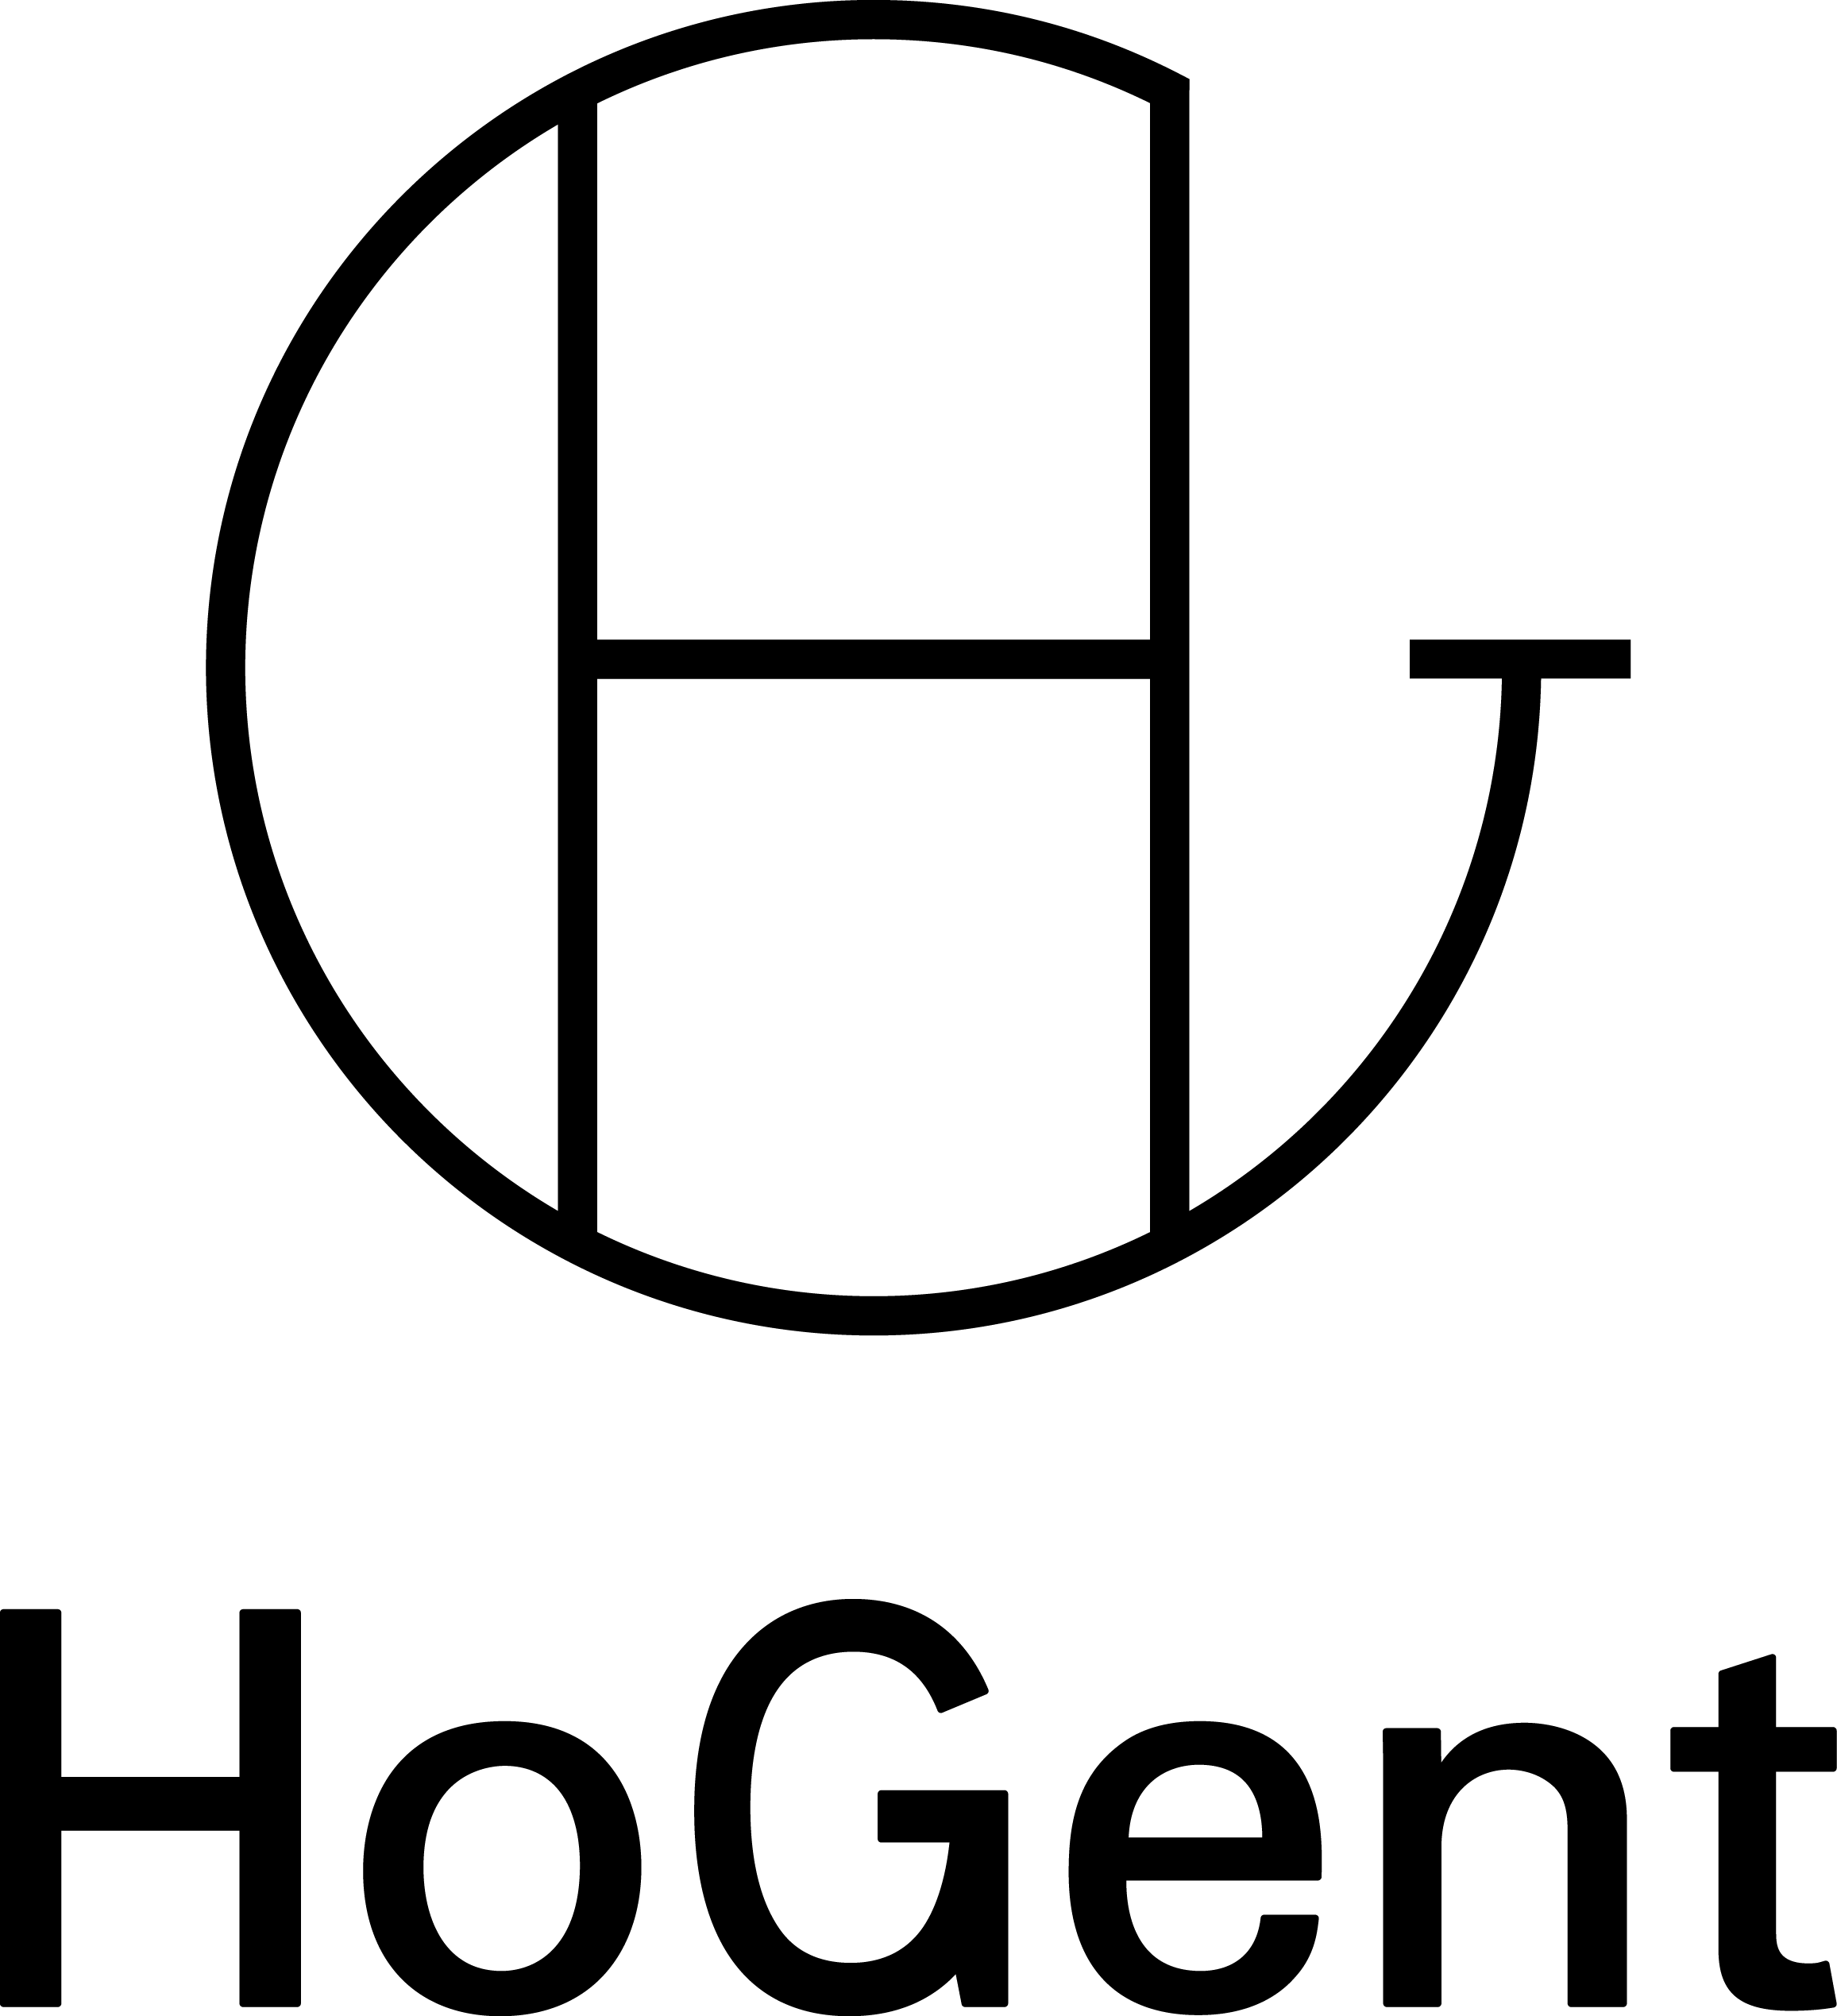
\includegraphics[width=2.5cm]{img/HG-beeldmerk-woordmerk}\\[.5cm]
    \faculteit\\[3cm]
    \titel
    \vfill
    \student\\[3.5cm]
    \rapporttype\\[2cm]
    Promotor:\\
    \promotor\\
    Co-promotor:\\
    \copromotor\\[2.5cm]
    Instelling: \instelling\\[.5cm]
    Academiejaar: \academiejaar\\[.5cm]
    \examenperiode
    \endgroup

  \end{center}
  \restoregeometry
\end{titlepage}

% Schutblad

\emptypage
\emptypage
\emptypage


\begin{titlepage}
  \newgeometry{top=5.35cm,bottom=1.5cm,left=1.5cm,right=1.5cm}
  \begin{center}

    \begingroup
    \rmfamily
    \faculty\\[3cm]
    \titleEN
    \vfill
    \student\\[3.5cm]
    \reporttype\\[2cm]
    Promotor:\\
    \promotor\\
    Co-promotor:\\
    \copromotor\\[2.5cm]
    Affiliation: \instelling\\[.5cm]
    Academic year: \academiejaar\\[.5cm]
    \examperiod
    \endgroup

  \end{center}
  \restoregeometry
\end{titlepage}

\emptypage

\begin{abstract}
Abstract in het Nederlands...
\end{abstract}

\emptypage

\begin{abstract}
The Internet of Things is today's buzzword when talking about future technology. A lot of companies are investing in this technology with new devices being made and added to the internet every day.

Around the same time of the release of IPv6, which provides a near inexhaustible number of IP addresses, Bluetooth Low Energy made it to the market as well. This technology aims to be the go-to technology when manufacturing low energy wearables and in the future, make it into the houses of everyone with updates like mesh networking which will help home automation.

With the massive growth of the Internet of Things, a huge opportunity arises since the wearables market is increasingly gaining traction as well. A lot of these wearables use Bluetooth Low Energy technology as a low power and cost-efficient data transfer technology.

This thesis aims to research Bluetooth Low Energy technology in a wearable context. The technology will be discussed as well as the difference between Bluetooth Low Energy and Bluetooth Classic. Further research includes the pros and cons, types of devices, the Bluetooth Low Energy protocol stack and more. A Proof of Concept will also be developed for an Android smartphone which aims to connect Bluetooth Low Energy wearables with the AllThingsTalk developer Cloud, which is one of the main goals for this thesis. Further goals include enabling real-time data transfer, supporting two-way data transfer and finding a real-life scenario where Bluetooth Low Energy wearables could provide an added value in an Internet of Things context.

In order to research these subjects, a general knowledge had to be gained about Bluetooth Low Energy. This technology was researched extensively in order to best prepare for the Proof of Concept. Besides the official Bluetooth Core Specification, some books were purchased by experts such as Kevin Townsend and Robin Heydon.

By putting the theory to the test in the Proof of Concept, we found that it is in fact possible to connect Bluetooth Low Energy wearables with a smartphone without too much trouble, as well as sending the data to an online Cloud where it can be analysed further.

In conclusion, it can be said that Bluetooth Low Energy is in fact a good technology for wearable devices. It consumes extremely little power and is easy to set up and support, as long as manufacturers use standard Bluetooth Profiles, since implementing custom profiles can get very complicated very quickly.

However, while the research questions have a fairly positive outcome, the Internet of Things still remains a big threat to a lot of people. Some problems concerning privacy and security arise, especially when dealing with sensitive objects.
\end{abstract}

\emptypage

\chapter*{Preface}
\label{ch:preface}
Technology has always been a huge interest of me. Whether it be computers, microcontrollers or simply fixing a radio, it is always fascinating to me how everything works and how little I seem to know the deeper I dig into things. A while ago I also got introduced to the world of Raspberry Pi and Arduino. I purchased an Arduino starter kit and started working on it and trying to understand it. It seemed to me that there was a lot more potential than just pressing a button that turns a light on, and it was around that time I discovered the Internet of Things. Back when I discovered it, the Internet of Things seemed like a huge thing that I could not wrap my head around and I did not know where to start until I got to my third year in college and had to pick a thesis subject. I wanted the thesis to reflect my interests, and at that time it was the Internet of Things.

After looking around for companies that were active in this field of work, I stumbled upon AllThingsTalk and asked if they had some potential research questions for me. After some mailing back and forth, Bluetooth Low Energy combined with wearables and Internet of Things came up and the subject immediately spoke to me as it seemed like an ideal combination of all my interests.

This thesis is the result of pouring most of my spare time into a subject that interests me a lot. It aims to be a guideline for people interested in Internet of Things, Bluetooth Low Energy and even companies that are doing research about Bluetooth Low Energy.

% TODO: Vergeet ook niet te bedanken wie je geholpen/gesteund/... heeft

\chapter*{Acknowledgements}
\label{ch:acknowledgements}
In the making of this thesis, a few people were indispensable into making it how it is now and they definitely deserve some words of gratitude. First of all I want to thank my promotor Joeri Van Herreweghe. He helped me a lot with the structural part of this thesis and provided tons of useful feedback every time I sent a draft to him. Next up I want to thank AllThingsTalk, in special Peter Leemans, who made this thesis possible by providing the excellent subject and all of the Bluetooth Low Energy devices that were used in the Proof of Concept, as well as great guidance throughout the semester with bi-weekly meetings. Furthermore I want to thank another member of AllThingsTalk, Jan Bogaerts, for assisting me on a more technical level for this thesis during our meetings and numerous emails. I also want to thank Thomas Clauwaert, Eva Emmerechts, Annemie De Groote, Lara Delange and Idriz Velghe. These people helped me with lots of different things like reviewing my English, reviewing the document structure and content, giving me moral support and helping me with a lot of little questions I had.

\tableofcontents

\emptypage

%%---------- Kern --------------------------------------------------------

\chapter{Introduction}
\label{ch:introduction}
\epigraph{``If you think that the internet has changed your life, think again. The IoT is about to change it all over again!''}{Brendan O'Brien}
The Internet of Things is a concept that has been around for quite some time, yet it is quickly becoming very popular and almost every company wants to be a part of it. It gained a lot of popularity around 2011 when IPv6 was released and it was around this time Gartner \citep{gartner2012} also took note of this trend and put it on their annual Hype Cycle for the first time. Around the same time of the growing popularity of the Internet of Things, the Bluetooth Special Interest Group released a new Bluetooth specification that was built for the Internet of Things: Bluetooth Low Energy. Gartner \citep{gartner2015} also suggests that by 2020, around 20 billion `things' will be connected to the Internet of Things, a market that Bluetooth Low Energy wants to play a big role in.

This thesis aims to provide an introduction to Bluetooth Low Energy and how a smartphone can be used as a gateway to allow Bluetooth Low Energy devices, which don't have internet capabilities, to connect to the internet. In this chapter the problem that the thesis is trying to find an answer for is elaborated, as well as the actual questions that need answering. An introduction about `AllThingsTalk' can also be found, a company that is trying to figure out how to connect Bluetooth Low Energy wearables with their Internet of Things infrastructure.

\newpage{}
\section{Problem statement and research questions}
\label{sec:problemdefinition}
First of all, the problem statement will be discussed where a quick sketch will be made as to why this thesis came to be. It will handle a subject that AllThingsTalk is very keen to discover for the development of their company and why combining Bluetooth Low Energy with their Internet of Things infrastructure is the next logical step for their business. Next, we'll look at the main questions AllThingsTalk wants an answer for together with some smaller questions that logically follow it.

\subsection{Problem statement}
\label{subsec:problemstatement}
At the time of writing, there are already a lot of internet enabled products on the market \citep{gartner2015}. With the new Bluetooth Low Energy specification, Bluetooth is reaching out to connect even more products to the smartphone and ultimately to the internet. These are products like socks\footnote{\url{http://www.sensoriafitness.com/}}, shoes\footnote{\url{https://secure-nikeplus.nike.com/plus/products/basketball}}, fitness bands\footnote{\url{https://www.fitbit.com/}} and more are being added to the list every day. The problem with these products is that in a lot of cases, the products only synchronize with a smartphone. Some manufacturers extend this connectivity by occasionally synchronizing the data the smartphone captures to their own proprietary Cloud, where the data can be analysed by both the company and the consumer. Most of the time, this is where the data cycle stops and it can't be further accessed by other parties, this is known as a closed loop system. In some cases, developers can still access the data with an API that communicates with the Cloud service of the manufacturer, but this doesn't give any access to the raw sensor values and doesn't allow real-time data transfer. Typically these Bluetooth Low Energy devices are built for the purpose of the (single) use case of the manufacturer. AllThingsTalk wants to find out how it can (re)use these existing devices for other use cases.

One of the use cases where low latency data communication through wearables could be useful is in elderly homes. For instance when making a monitoring system to check if elderly people have fallen by tracking the gyroscope and accelerometer of a wearable, it is not acceptable to receive data every 15 minutes because by that time help might be too late when considering a worst case scenario. When building a system like this, it can also be useful to have a central service where all of the raw data is collected instead of containing it in multiple closed loops for every device of a different manufacturer. While a closed system is an approach that could work, it does not give as much flexibility over all of the data compared to an open system and few manufacturers expose this data for further use. An example of a closed system versus open system can be found in figure \ref{fig:networkloops}.

On top of this, a lot of the Bluetooth Low Energy wearables being manufactured don't use Bluetooth Special Interest Group adopted standards, which makes interoperability with existing applications hard, if not impossible if authentication and encryption are added into the mix.

\begin{figure}[h]
    \centering
    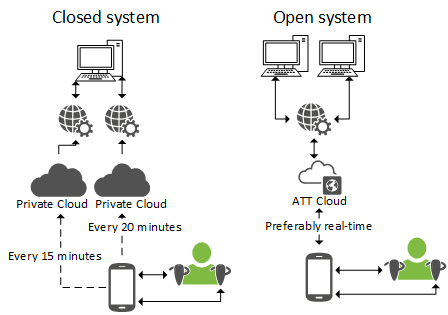
\includegraphics[width=0.9\textwidth]{img/networkloop.png}
    \caption[Image demonstrating a closed Cloud system versus an open Cloud system]{Image demonstrating a closed system (left) versus an open system (right). A closed system usually has its own (optional) Cloud for every device from a different manufacturer, where the smartphone only pushes data to the Cloud but rarely pulls it for further use. It also (not always) exposes a web service to allow users to pull the data to their computer. An open system exposes \textit{one} public Cloud like the AllThingsTalk developer Cloud with \textit{one} web service, also allowing 2-way data communication between smartphone and Cloud.}
    \label{fig:networkloops}
\end{figure}

\subsection{Research questions}
\label{subsec:researchquestions}
There are a couple of questions that can be asked when combining Bluetooth Low Energy and the Internet of Things, and some of those questions alone could have multiple papers dedicated to them. For example, the matter of security will be a never ending debate, and even more concerns arise when talking about security in the Internet of Things. Another issue is privacy, but since this is very much a grey area it is hard to formulate a one-sided conclusion on this matter. Some of these concerns will be addressed further in section \ref{sec:concerns}.

The main goals this thesis is aiming to fulfil are in essence very simple, but there are always some other questions that arise when looking at the big picture. These questions can be categorized as followed, the questions in bold being the main research questions and the ones in plain text being auxiliary questions:
\begin{itemize}
	\item{\textbf{Can Bluetooth Low Energy wearables be used in an Internet of Things Cloud infrastructure?}}
	\item{\textbf{Is is possible to use a smartphone as a gateway to communicate with the AllThingsTalk developer Cloud in real-time?}}
	\item{\textbf{Is there a possible use case where Bluetooth Low Energy wearables can provide an added value in an Internet of Things use case?}}
	\item{What is Bluetooth Low Energy?}
	\item{What is the difference between Bluetooth Low Energy and Bluetooth Classic?}
	\item{What are the pros and cons of this technology?}
	\item{What types of devices exist in Bluetooth Low Energy and how do they expose their data?}
\end{itemize}

\section{AllThingsTalk}
\label{sec:allthingstalk}
AllThingsTalk has been referenced a couple of times in the previous section and will be referenced some more in the remainder of this paper. The reason for this is that this thesis is affiliated with this company and is being written for them. The company helped shape the vision of the thesis and offered some very interesting insights and ideas for subjects to write about, subjects which were very interesting for internal use in the company.

AllThingsTalk was founded in July 2013 and their main objective is to `Make IoT ideas happen'. The company is already counting thirteen employees in two different countries, the headquarters being located in Ghent, Belgium. The office in Belgium counts seven people and is heavily focused on research \& development engineering, project management and sales \& marketing. The branch office is located in Belgrade, Serbia with the other six people, and their main focus is platform software development.

\subsection{History}
\label{subsec:atthistory}
AllThingsTalk has come a long way since the start of the company. They have received multiple Research \& Innovation grants from the government, the first being in September 2013 for building an open IoT platform: the AllThingsTalk developer Cloud. The second grant was received in May 2014, where the goal was to implement pattern recognition in their platform. A third grant was acquired in February 2015, which was responsible for adding machine learning components to the platform.

Furthermore, they have hit some other major milestones throughout the years. In November 2014 they launched the first set of Rapid Development Kits for Internet of Things, where they added the Intel Rapid Development Kit in April 2015 and the LoRa Rapid Development Kit in November 2015. Other milestones include Internet of Things hackathons, the launch of \url{IOTOPIA.be} - a platform to introduce children in secondary schools to Internet of Things - and a LoRa partnership with Proximus, a telecommunications company in Belgium.

\subsection{Products and services}
\label{subsec:attproductsservices}
The three main products and services AllThingsTalk offer are guidance, tools and Cloud. 

For guidance, they offer IoT innovation workshops and private hackathons. This means that AllThingstalk organizes workshops for companies tailored to their needs, as well as hackathons which involve ideation, prototyping and more.

The second product is tools. AllThingsTalk offers a range of development kits that companies can purchase to accelerate their Internet of Things research. This includes kits like LoRa, Arduino, Raspberry Pi, Intel Edison and Windows 10 IoT. `Hackathon in a Box' is also available, which helps companies to organize their own Internet of Things hackathon on their own.

Last but not least is the AllThingsTalk developer Cloud, an Internet of Things prototyping platform which enables companies to connect their devices rapidly to the Cloud, instead of hosting their own complicated infrastructure. Not only can this be used to prototype, but the platform is already being used in some very exciting projects like helping the elderly live in their home longer and an ongoing project which provides predictive maintenance in industries with machinery.

\chapter{Methodology}
\label{ch:methodology}
\epigraph{``Research is formalized curiosity. It is poking and prying with a purpose.''}{Zora Neale Hurston}
This chapter aims to elaborate what approaches and methods were used in the making of this thesis. It explains what methods were used for the two major parts of this thesis, being the research \& literature study and the Proof of Concept.

\section{Research and literature study}
\label{sec:researchlit}
Before starting the research, the most important question was `what does AllThingsTalk already know?'. Being a company revolving around Internet of Things, it would not be of much use to dedicate a large portion of this paper to it. However, some research had to be done about Internet of Things in order to understand some core concepts and technologies that are used like transfer protocols such as MQTT and AMQP. A more abstract understanding was also needed, being how the Internet of Things works, what it is used for, why it is important... . This information is easily found online and since it is not the main purpose of this thesis, it was not included.

That being said, the core subject of the research and literature study is about Bluetooth Low Energy. The research about this technology was done like any other subject would be researched: start at the basics and work up to more advanced cases. Initially, the plan was to rely heavily on the official documentation of Bluetooth \citep{bluetooth2014bluetooth}, but since the complete Bluetooth specification is over 2000 pages in length, a more practical approach was to purchase books that explain Bluetooth Low Energy, two of them being \cite{Townsend2014} and \cite{heydon2012bluetooth} and going back to the documentation when extra information was needed.

There are also training videos to be found on the Bluetooth website as well as various other short introductions to the technology all over the web, which provide a basic and quick understanding about the technology.

\section{Proof of Concept}
\label{sec:poc}
One of the biggest focuses of the Proof of Concept was to simply try out the technology and putting the theory to use. The actual goals of the Proof of Concept were more to provide the Bluetooth Low Energy layer than to connect to the internet, as AllThingsTalk provides easy-to-use libraries in various programming languages to connect to their platform. Another reason for the Proof of Concept was to prove that a smartphone can be used as a gateway to connect Bluetooth Low Energy wearables to the Cloud and that it can provide an added value in a real life scenario. By accomplishing this, it should provide a clear answer to the main research questions defined in subsection \ref{subsec:researchquestions}.

In order to help speed up the learning process and quickly allow me to prototype and try out the technology, various devices were provided by AllThingsTalk which offer a range of Bluetooth Low Energy Profiles, Services and Characteristics (explained in chapter \ref{ch:gatt}). The devices that were used and what things were accomplished with them will be discussed in chapter \ref{ch:android}.

The first goal of the Proof of Concept was to connect to a Bluetooth Low Energy device and read data with a smartphone. Various examples and repositories with source code provided some interesting insights as to how this Android API works. Bluetooth also offers some starter kits to kick-start any project that wants to use Bluetooth Low Energy, including a very comprehensive and easy to use wrapper around the Android Bluetooth API.

Further goals include writing data and coupling the Bluetooth layer to the network layer, automatic Service discovery and mapping, automatic generation of assets on the online platform and more. The most important concepts on how to achieve this are elaborated in chapter \ref{ch:android} and the accomplishments of both the literature study and Proof of Concept are listed in section \ref{sec:conclusion}.


% TODO: Hoe ben je te werk gegaan? Verdeel je onderzoek in grote fasen, en
% licht in elke fase toe welke stappen je gevolgd hebt. Verantwoord waarom je
% op deze manier te werk gegaan bent. Je moet kunnen aantonen dat je de best
% mogelijke manier toegepast hebt om een antwoord te vinden op de
% onderzoeksvraag.


%% TODO: de structuur en titel van deze hoofdstukken hangen af van je 
% eigen onderzoek. Elke fase in je onderzoek kan een eigen hoofdstuk krijgen. Kies telkens een gepaste titel. ``Corpus'' is *GEEN* gepaste titel
\chapter{Bluetooth Low Energy}
\label{ch:ble}
\epigraph{``Bluetooth Low Energy is going to change the way the world connects.''}{Robin Heydon}
Bluetooth has been around for about 16 years and with the adoption of Bluetooth Low Energy in 2010, it seems like it is going to be around for a little while longer \citep{bluetoothsig2016}. Originally known as Wibree by Nokia \citep{nokia2006}, it was later merged into the Bluetooth standard. This technology was designed from the ground up \citep{gupta2013inside} to be as energy efficient as possible and wants to power the Internet of Things for years to come. Exciting updates are also on the way like mesh networking, allowing different nodes in a network to relay data to one another. In this chapter a closer look will be taken at Bluetooth Low Energy and what the key differences are between Bluetooth BR/EDR\footnote{Basic Rate/Enhanced Data Rate, ``normal'' Bluetooth} and Bluetooth Low Energy. Also worth investigating are the limitations of Bluetooth Low Energy and how this technology achieves low energy like no other when compared to similar technologies like Zigbee \citep{siekkinen2012low}.

\newpage{}

\section{What is Bluetooth Low Energy}
\label{sec:whatis}
In essence, Bluetooth Low Energy is an open standard that consumes extremely low power. It has been designed from scratch and has more things not in common than it does with Bluetooth, so the name can be a little bit confusing. Every component in this specification has been designed to consume as little power as possible, that's why this technology can also be called a `coin cell' technology \citep{bluetooth2016training}. It is called a coin cell technology because a Bluetooth Low Energy enabled device can (theoretically, with normal usage) achieve a battery life of around eight months on a coin cell battery. A great example of this are beacons, which can achieve very long battery life if configured correctly. If fitted with a bigger battery, it can last for over two years. More information about the battery usage and how low energy is achieved can be found in section \ref{sec:lowenergy}.

However, one might think: ``if Bluetooth Low Energy is so great, why isn't it replacing other wireless technologies?''. The main reason for this is because it is very slow and has very little range. A couple of other limitations are present, but these will be more closely looked at in subsection \ref{subsec:limitations}. Bluetooth Low Energy's main use is intended for Personal Area Networks with a gateway in range that can relay data to a Cloud service in order to connect various devices together.

\section{Key differences between classic Bluetooth}
\label{sec:differencesclassic}
It seems that Bluetooth and Bluetooth Low Energy are worlds apart from one another. This is in fact very correct so it is hard to just list some differences and be done with it. In the next two subsections we'll look at why Bluetooth Low Energy is completely different from Bluetooth and should be seen as an entirely new technology instead of an enhancement to the Bluetooth Classic specification. The key limitations of the Bluetooth Low Energy specification are also addressed further in this section.

\subsection{A new technology emerges}
\label{subsec:newtechnology}
A lot of authors are looking to compare Bluetooth with Bluetooth Low Energy, but this is an unfair comparison since the use cases for both of these technologies are completely different. As the name suggests, Bluetooth Low Energy is marketed for low energy devices like wearables and sensors, so it isn't here to replace other wireless technologies in the slightest. They've also both been built around completely different core principles and have been designed to fulfil these requirements as best as possible.

\subsection{Limitations of Bluetooth Low Energy}
\label{subsec:limitations}
Bluetooth Low Energy does not bring all good news as there are a few key limitations to the technology. Because the technology uses very little power, it is fairly easy to understand that the transmit power and transfer speeds are not anywhere near technologies like Wi-Fi or 4G-LTE. In theory, Bluetooth Low Energy can achieve ranges of up to 65 meters and upcoming updates to the specification prove that this range will be increased even more \citep{heydon2012bluetooth}. However, most manufacturers won't want their peripheral to transmit at such high range because this will cause increased battery usage in turn. In practice, this range is much lower as walls and even humans can interfere with transmission range \citep{faragher2014analysis}.

Another limitation is the transfer speed. Again, in theory, Bluetooth Low Energy can have a (full packet) transfer speed of up to 1 Mbps\footnote{1 Mbps equals to 100 kilobytes per second.}. If the useful data contained in said packet is taken into account and all of the overhead that goes into transferring, encoding and decoding a packet is added up, 5 to 10 KB per second is a much more realistic representation. Knowing this, it is safe to assume that Bluetooth Low Energy won't be replacing Wi-Fi any time soon.

A more concerning limitation is that Bluetooth Low Energy operates in the 2.4 GHz ISM frequency band, the same band that Wi-Fi uses. They've chosen this band because the 2.4 GHz ISM band does not require any licensing cost, contributing to the very low chip cost of Bluetooth Low Energy devices. Luckily, Bluetooth Low Energy features an algorithm to avoid major interference from Wi-Fi, as it will avoid any channel that is being heavily used by other wireless technologies.

\section{Bluetooth configurations}
\label{sec:bleconfigurations}
Bluetooth Low Energy is known by a variety of names on the market and while some of them are used to describe the same technology, in a few there are some differences to be found. `Bluetooth Low Energy' is mostly used as a catch-all name and can consist of a few different configurations. Some people assume Bluetooth BR/EDR is also Bluetooth Low Energy, but this assumption could not be more wrong. If there is a product that specifies that a smartphone must have Bluetooth Version 4.0 or later, that product is probably a Bluetooth Low Energy device.

Other names that can commonly be found are Bluetooth Smart (single-mode) and Bluetooth Smart Ready (dual-mode), these are both specifications of Bluetooth Low Energy but still have differences between them \citep{Townsend2014}. Bluetooth Smart has been designed to only allow interoperability between other Bluetooth Smart products and Bluetooth Smart Ready products. This configuration will usually be seen in wearable devices that connect to a smartphone, in this case the wearable is a Bluetooth Smart product and the smartphone is a Bluetooth Smart Ready product. Bluetooth Smart Ready on the other hand has been designed to allow communication with Bluetooth, Bluetooth Smart Ready and Bluetooth Smart products. Bluetooth Smart Ready is commonly present in the most recent smartphones, which will allow communication with Bluetooth products like headphones but also Bluetooth Smart products like a smart band. A more comprehensible and orderly overview of these technologies can be found in table \ref{table:configurations}.

\begin{table}[]
\centering
\caption[Compatibility table of Bluetooth specifications]{Compatibility table of Bluetooth specifications \citep{Townsend2014}}
\label{table:configurations}
\begin{tabular}{|l|l|l|}
\hline
\textit{\textbf{Bluetooth specification}} & \textit{\textbf{Supports BR/EDR}} & \textit{\textbf{Supports BLE}} \\ \hline
\textbf{Pre-v4.0}                   & yes                                 & no                              \\ \hline
\textbf{4.x Bluetooth Smart}        & no                                  & yes                              \\ \hline
\textbf{4.x Bluetooth Smart Ready}  & yes                                 & yes                              \\ \hline
\end{tabular}
\end{table}

\section{How low energy is achieved}
\label{sec:lowenergy}
There are a couple of techniques Bluetooth Low Energy uses to achieve low energy consumption. The fact alone that it can run off a 3 volt CR2032 coin cell battery and still retain one year of battery life \citep{kamath2010measuring} proves that it is indeed a \textit{true} low energy technology. There are a couple of decisions that made it possible to achieve this low amount of energy consumption, some being the following:

\begin{itemize}
\item{\textbf{Use the radio as little as possible.} Keeping the radio for any wireless technology active requires power, which is also the case with Bluetooth Low Energy. By using the radio as little as possible, Bluetooth Low Energy can significantly increase its battery life. At a set interval, devices will broadcast advertising packets on the three advertising channels, which are explained more in section \ref{sec:channels}. After it advertises, it must listen briefly to any connection requests that follow it, in between these events the radio is simply turned off. The radio and the protocol stack, explained more in depth in chapter \ref{ch:protocolstack}, have also been designed to be as fast as possible. An advertising event, connection event, reading a single value of data and acknowledging the event can take as little as 3 milliseconds \citep{heydon2012bluetooth}, which is vital in not only keeping the energy consumption to a minimum, but it also helps passively cool the radio.}

\item{\textbf{Keep packets very small.} Restricting the packet length to a maximum of 47 bytes allows very rapid packet transfers, which in turn contributes to keeping the radio off as much as possible. Keeping packets small also lowers the complexity of the transmitter and receiver, resulting in much lower power consumption than technologies that allow large packets.}
\end{itemize}

\chapter{The Bluetooth Low Energy protocol stack}
\label{ch:protocolstack}
\epigraph{``The real danger is not that computers will begin to think like men, but that men will begin to think like computers.''}{Sydney Harris}
Before diving more into the specifics about communication in Bluetooth Low Energy with data packets and advertising packets it is important to know at least some of the fundamentals of the protocol stack that enables devices to communicate with one another. The protocol stack consists of three main parts: the controller, the host and the application. In this chapter each of the layers, interfaces, protocols and profiles that make up these three parts will be looked at, giving some insights as to how Bluetooth Low Energy works on a lower level and how data is delegated from layer to layer to build comprehensible communication. Two of the profiles discussed in this chapter however are a fundamental part of Bluetooth Low Energy and thus have their own chapters dedicated to them in order to go into them deeper.

\newpage{}

\section{Controller}
\label{sec:stackController}
At the lowest level in the Bluetooth Low Energy stack, closest to the actual antenna which sends packets, is the Controller. The Controller manages a couple of things like sending raw data through the radio and governing the state of the radio, but its tasks definitely don't end there. In the following subsections the Physical Layer, Link layer and Host Controller Interface will be looked at, which are vital components in the low level communication of Bluetooth Low Energy.

\subsection{Physical Layer}
\label{subsec:controllerPHY}
The Physical Layer is the layer responsible for actually sending data over the air. As explained in section \ref{sec:channels}, the physical layer uses the 2.4 GHz ISM band to send and receive its data. In order to avoid interference from Wi-Fi or other technologies that use this band, Bluetooth Low Energy uses frequency hopping with the following formula:

\begin{equation*}
\text{newChannel = (currentChannel + hopAmount) mod 37}
\end{equation*}

The hop amount is communicated with both master and slave once a connection has been established, so this hop amount can be different for every connection made and it shouldn't be assumed that this is a fixed number. A modulo of 37 is taken from the sum because Bluetooth Low Energy has 37 channels available for connections, as shown in figure \ref{fig:channelmap}.

\subsection{Link Layer}
\label{subsec:controllerLL}
The Link Layer is the layer that manages the Physical Layer. It governs the data the Physical Layer should send and it also keeps the state of the Physical Layer in order, the state machine diagram is shown in figure \ref{fig:llstatemachine}. 

This state machine diagram shows which states the Physical Layer can be in. The Physical Layer can only be in one state at a time, and the diagram shows which states each state can flow into when it is finished.

First up is the Standby state, where the Physical Layer doesn't send nor receive any packets. As seen on the diagram, the Standby state can be entered from any other state and can transition into any state except the Connection state.

In the Advertising state, the Physical Layer will only advertise its presence and potential sensor data if configured correctly, this is also known as an advertiser. It also listens to scan requests and can respond to these requests if it wishes to do so. This state can only be entered from the Standby state.

Next up is the Scanning state, where the Physical Layer only listens to advertising packets from other Bluetooth Low Energy devices, this is also known as a Scanner. The Scanning state can only be entered from the Standby state.

Further up is the Initiating state, where the Physical Layer listens to advertising packets from certain devices which have indicated they want to connect to the device, this is also known as an Initiator. The Initiating state can only be entered from the Standby state after the right conditions have been met.

Last but not least is the Connection state. This state can be entered from both the Advertising and Initiating state. When it is entered from the Advertising state, the device will take on the role of slave or peripheral. When entered from the Initiating state, the device will be seen as the master.

\begin{figure}[h]
    \centering
    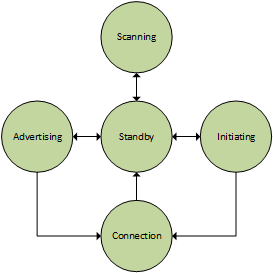
\includegraphics[width=0.5\textwidth]{img/llstate.png}
    \caption[State diagram for the Link Layer state machine]{State diagram for the Link Layer state machine. Based on the state machine shown at \url{https://www.bluetooth.com/specifications/bluetooth-core-specification/technical-considerations}}
    \label{fig:llstatemachine}
\end{figure}

\subsection{Host Controller Interface}
\label{subsec:controllerHCI}
The Host Controller Interface provides interfaces so the Host can more easily communicate with the Controller. This was a common architecture in Bluetooth Classic so Bluetooth Low Energy has also adopted this way of working. The Host Controller Interface has to be present on both the Host and Controller level, providing a channel where everything can be routed through. This makes it possible to separate the Host and Controller from one another, which is the case in many mobile devices like a smartphone. The Host part will typically be handled by the smartphone itself, but the actual Bluetooth hardware and Controller are embedded in a different chip. It is also possible to host the entire Bluetooth Low Energy stack on a single chip, which is usually the case with sensors or other low power devices.

There are a couple of different interfaces that are used commonly on different types of devices. On a device with a lot of power  USB\footnote{Universal Serial Bus} is commonly used but on lower powered devices, a UART\footnote{Universal Asynchronous Receiver/Transmitter} interface is typically provided but an SDIO\footnote{Secure Digital Input Output} interface can also be used.

\section{Host}
\label{sec:stackHost}
Above the Controller resides the Host, which is built on top of the Host side of the Host Controller Interface. The Host contains quite a lot of different layers, protocols and procedures exposed as an API to allow the Application to easily tap into this functionality.

\subsection{Host Controller Interface}
\label{subsec:hostHCI}
The Host side of the Host Controller Interface is pretty much the same as the Controller side. It is simply a layer in between the Host and the Controller, where the Host side exposes different interfaces to send data to and the Controller side will then control the hardware to do the right thing and make sure the data gets sent correctly.

\subsection{Logical Link Control and Adaptation Protocol}
\label{subsec:hostL2CAP}
The Logical Link Control and Adaptation Protocol, or L2CAP in short, is the layer that provides multiplexing capabilities to the Bluetooth Low Energy stack. Multiplexing provides a way to encapsulate different protocols and messages into a single Bluetooth Low Energy data packet and can also convert them back when receiving a packet.

If the data sent by the upper layers in the stack is too large, L2CAP can also split this data into the maximum size of a payload. Naturally, it can also gather multiple fragmented packets it receives and combine them again for processing.

\subsection{Attribute Protocol}
\label{subsec:hostATT}
The Attribute Protocol is responsible for exposing a ``database'' with attributes and their respective values, permissions, handles and unique identifiers. The peripheral that exposes this database is called a server and the device requesting values is called a client. The client can use the attribute handle to request data for the given attribute.

\subsection{Security Manager Protocol}
\label{subsec:hostSMP}
As the name suggests, the Security Manager Protocol handles all of the security for a Bluetooth Low Energy device. It is used for the very common ``pairing'' action for Bluetooth devices. This action pairs two devices together with randomized keys, allowing easy reconnection in the future. The Security Manager Protocol is responsible for generating and handing out these keys. It is also responsible for encrypting the link if the client requests to do so.

\subsection{Generic Access Profile}
\label{subsec:hostGAP}
The Generic Access Profile, as it is conveniently named, manages all of the access to the device. It provides functionality for advertising device presence, allowing other devices to scan it and then read the advertising packet payload or initiate a connection request. This profile also defines behaviour once devices are connected and some procedures that allow extra security measures. In-depth information about the Generic Access Profile will be given in chapter \ref{ch:gap}.

\subsection{Generic Attribute Profile}
\label{subsec:hostGATT}
The Generic Attribute Profile or GATT is the layer above the Attribute Protocol. While the Attribute Protocol exposes an attribute server, GATT provides a layer of abstraction above these attributes, grouping them into Services and Characteristics. It also enables Services to contain other Services. More information about GATT is given in chapter \ref{ch:gatt}.

\section{Application}
\label{sec:stackApplication}
At the highest level of the protocol stack is the Application. The Application is the actual program that contains logic, calculations and/or the user interface. Some of these Applications are standards defined by the Bluetooth Special Interest Group as Profiles, but custom Profiles could also be developed. It would be up to the manufacturer to expose these Profiles to allow interoperability with other devices.

\chapter{Generic Access Profile}
\label{ch:gap}
\epigraph{``Once a new technology rolls over you, if you’re not part of the steamroller, you’re part of the road.''}{Stewart Brand}
One of the most basic components in Bluetooth Low Energy is the Generic Access Profile \citep{heydon2012bluetooth}. This profile determines everything from advertising device presence to continuing to a connection. It specifies rules how devices can and must behave in order to interact with one another and imposes some general rules devices have to follow. It also supports some modes and procedures to secure the data link like authentication, bonding, authorization and encryption. In this chapter, some general information about the Generic Access Profile like device roles and data channels will be looked at before describing how advertising, scanning, broadcasting and connections work.

\newpage{}

\section{Roles}
\label{sec:roles}
Every Bluetooth Low Energy device has one or more roles it can fulfil. Each of these roles has been optimized to perform their task as best it can. First of all there's the Broadcaster role, which only requires a device to have a transmitter and advertising profile. Broadcasters aren't necessarily devices that can be connected to, so manufacturing broadcast only devices could cut down on cost even more as there's no need to have a receiver on these devices. An example of this is a thermostat which constantly broadcasts its temperature.

Secondly there's the Observers, these devices are opposite to broadcasters as they don't require a transmitter. Observers just listen to advertising events and process the data further, without ever making a connection. These devices make perfect gateways for Broadcasters, as a connection will never occur between these two, and the Observer can just relay the data to another collection point.

The last two roles are Peripherals and Centrals. These two are the most complex roles as both devices are required to have both a transmitter and receiver. The big difference however is that a Peripheral will always act as a slave in a connection and a Central will always act as a master. This also means that the peripheral will (most of the time) be the least powerful device with the lowest battery life, like a watch or a sensor. It is vital that Peripheral devices do not do the heavy lifting in connections because this would drain the battery too fast. The Central in a connection is usually a more powerful device with better battery life, like a smartphone, tablet or even computers.

\section{Data channels}
\label{sec:channels}
Bluetooth Low Energy uses a number of channels in the 2.4 GHz ISM frequency band. Some of these channels are used for advertising and most of them are used for transferring data once a connection has been made. Bluetooth Low Energy uses 40 channels to transmit data, 3 of which are used for advertising and the remaining 37 are used for connections. The frequency range starts at 2402 MHz and ends at 2483.5 MHz, giving each frequency a range of about 2 MHz to operate on. These channels have been carefully picked to have the least interference possible from Wi-Fi on the advertising channels. Since every connection starts with advertisements it is vital that these packets flow without interference. A visualization of these channels can be found in figure \ref{fig:channelmap}. The green channels are advertising channels while the remaining 37 are used for connections. LL stands for the corresponding number that the Link Layer assigns to these channels.

In order to make sure that connection packets flow as frequently as possible without having too many dropped packets, Bluetooth Low Energy uses adaptive frequency hopping. This means that at a set interval that the master and slave negotiate with each other, they will switch frequency with a negotiated hop amount, ensuring they'll always end up in the same frequency band. If data doesn't make it through on a given channel, the frequency hop will occur prematurely and both master and slave will move on to the next frequency and resend the packet(s) that weren't acknowledged.

\begin{figure}[h]
    \centering
    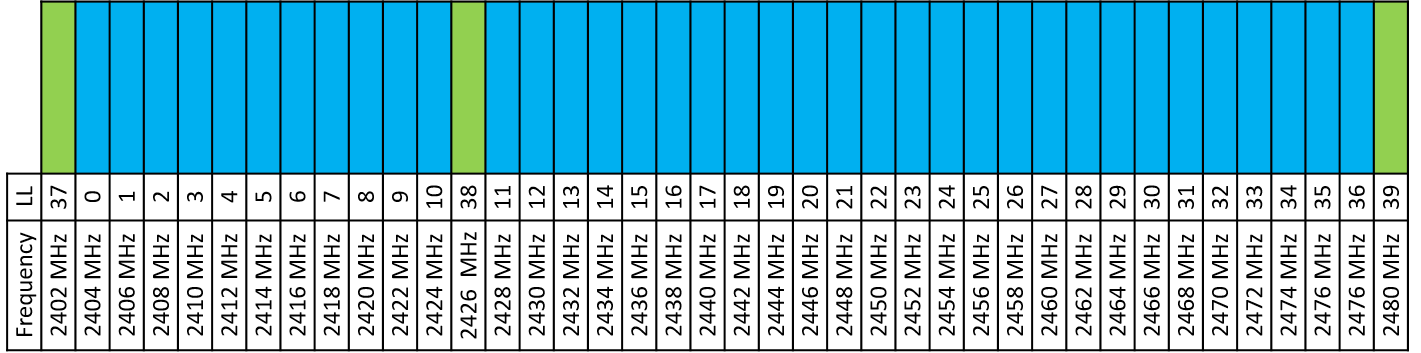
\includegraphics[width=0.9\textwidth]{img/channelmap.png}
    \caption[Image visualizing the Bluetooth Low Energy channel spectrum]{Image visualizing the Bluetooth Low Energy channel spectrum. Based on \cite{Townsend2014}.}
    \label{fig:channelmap}
\end{figure}

\section{Advertising}
\label{sec:advertising}
As quoted a few times before, advertising is one of the most important procedures in Bluetooth Low Energy. A device can be built solely around advertising data, but no device can work without it. Its main purpose is to broadcast the device is present and active so other devices can connect with it, but it can be used for more than that. A typical device will constantly be advertising its state to other devices. This state can be device name, device address and even an (incomplete) list of available Services on the device. The advertising interval differs from device to device, but it is easy to conclude that a device with a faster advertising interval will drain battery more quickly than one with a slow advertising interval.

If the device can't fit enough data into the advertising packet, there is a second option to send more data without requiring a connection. Once a device receives an advertising packet, it can send out a Scan Request, acknowledging that it received the previous advertising packet and is listening for extra packets if there are any. The peripheral can then proceed to send a Scan Response with extra data.

\subsection{Data format}
\label{subsec:advdataformat}
As discussed in subsection \ref{subsec:controllerLL}, each packet, be it advertising or data, has the same maximum length and structure but the data part of the packet is filled depending on the type of packet that is sent. The data in an advertising packet is filled with AD Types which take up one byte, and the data for that AD Type which is of variable length. An incomplete list of these AD Types together with their definition is found below. A full list of AD Types together with their descriptions can be found on the Bluetooth website\footnote{\url{https://www.bluetooth.com/specifications/assigned-numbers/generic-access-profile}} and Bluetooth Core Specification \citep{bluetooth2014bluetooth}.

\begin{itemize}
	\item {List of Service Class UUIDs (0x02 - 0x07): Helps with finding out the purpose of a device, can contain a complete or partial list of available Services on the device.}
	\item {Shortened or Complete Local Name (0x08 \& 0x09): Usually gives a friendly name to a device in UTF-8 format.}
	\item {Service Data (0x16): Represents a GATT Service and the data associated with it, this is in essence how a broadcasting only device transfers data.}
	\item {Appearance (0x19): Contains a number representing the external appearance. This can be anything from ``Generic Keyring'' to ``Joystick''.}
	\item {Indoor Positioning (0x25): Helps with mapping Bluetooth Low Energy devices in a building, can contain coordinates, altitude, floor number and location name.}
	\item {Advertising Interval (0x1A): How often the device advertises its presence.}
\end{itemize}

\section{Broadcasting}
\label{sec:broadcasting}
As discussed in section \ref{sec:advertising}, it is possible to have a device that only advertises data and isn't connectable, or its main purpose does not rely on connections. This is known as a broadcast device and can be used in broadcasting network topologies. Take for example a radio station, it simply broadcasts its data and it does not really matter how many people are listening. When broadcasting, an unlimited amount of devices can be listening to the data stream and security usually is not implemented here because advertising packets should not contain sensitive data. A great example of this are beacons, which constantly broadcast a very simple payload telling they are there. Once sensitive data needs to be sent or when two-way communication is the main use case, a connection should be established which uses the GATT Profile to exchange data between master and slave. More information on GATT can be found in chapter \ref{ch:gatt}.

\section{Connections}
\label{sec:connections}
Once a central is ready to connect to a peripheral, it sends a connection request to the peripheral. The peripheral can then accept or deny the request and once accepted, the connection sequence can begin. During the establishment of a connection, a few key rules are established that will stay in place for the remainder of that connection or until both devices agree to change the connection parameters. These rules can be hop frequency, hop amount, what to do when the connection fails and more. Some of these parameters can be changed during the connection lifetime, an example of this is given in section \ref{sec:channels}, where the devices can agree to avoid a given channel for a certain time because there is too much interference. Once a connection has been established, the peripheral will stop advertising its presence since it can only be connected to one central. For the remainder of that connection, both master and slave will exchange data solely with GATT until the connection terminates. The peripheral will then continue once again to advertise its presence.

\chapter{Generic Attribute Profile}
\label{ch:gatt}
\epigraph{``You can have data without information, but you cannot have information without data.''}{Daniel Keys Moran}
At the core of Bluetooth Low Energy communication is the Generic Attribute Profile or GATT \citep{Townsend2014}. It is something a client will use in every data request or data push once a dedicated connection has been set up. It defines the way data is transferred in Bluetooth Low Energy and it uses the Attribute protocol, which is the protocol that stores all of the attributes of a given device. In this chapter the general Attribute Profile and Protocol will be discussed, as well as the different data structures that come in to play. An example of an Attribute server will also be given using a standard SIG-approved Profile, as well as why and how one would implement their own Profile, either because the SIG-approved Profiles don't fit the use case or because the manufacturer wants to make the used technology more private.

\newpage{}

\section{Profiles}
\label{sec:profiles}
Profiles in Bluetooth Low Energy are an abstract representation of how a device can be implemented to fill a specific use case. These profiles are purely an example of how things can be done and these can be extended for every use case or a new profile can be made from scratch. The Heart Rate Profile for example defines that the device uses a minimum of two Services: the Heart Rate Service and the Device Information Service. Its role is a Heart Rate Sensor and it can broadcast its data or send it to a master device once a connection has been made.

\section{Services}
\label{sec:services}
All data in Bluetooth Low Energy is accessed through Services. It can be compared to simple Object Oriented principles: a Service has multiple Characteristics and a Characteristic belongs to one single Service. An example of this is the Bluetooth SIG defined Heart Rate Service. This document defines the way the Heart Rate Service is used and what Characteristics are contained in the Service. For example, the Heart Rate Service defines 3 Characteristics: Heart Rate Measurement, Body Sensor Location and Heart Rate Control Point, only the Heart Rate Measurement is mandatory to include. A functioning Arduino application serving a Heart Rate Service together with a custom written Service can be found in Appendix \ref{ch:arduinosketch}.

A device can host any number of Services which are independent of one another. Every Service also has its own security options which can be customized. Options like encryption for individual Services or the device as a whole can be set.

Apart from multiple primary Services, a Service can also be contained in a parent Service, this is then known as a secondary Service. However, the secondary Service approach isn't encountered that often, but it can be useful at times. Take for example a device which has two temperature sensors, one for the outside temperature and one for the battery temperature. The manufacturer could then choose to include the temperature Service for the battery as a secondary Service of the battery Service, this avoids ambiguity.

Apart from the SIG-defined Services, a custom Service can be designed if the defined Services don't meet the expectations of the use case. It is up to the manufacturer to provide documentation for these Services or not.

\section{Characteristics}
\label{sec:characteristics}
The actual data of Services is contained in Characteristics. Every Characteristic belongs to a specific Service and has a value attached to it. However, just because the Characteristic can be seen doesn't mean that it doesn't need any rights to read or write it. A Characteristic can specify certain rights like read, write, read uncommitted (where no acknowledgement is sent for the write request) and more. This is something that can be ignored, but an error message will be returned anyway if a device tries to read a Characteristic that isn't readable. These permissions can be used to notify the user interface that it shouldn't allow the user to interact with certain Characteristics.

If we take our trusty Heart Rate for example, the Heart Rate Measurement, we can look at the data structure and how the value should be parsed. This Characteristic also has some ``Flags'' bits which indicate things like the data type of the value (UINT8 or UINT16) and if certain fields are present or not. Depending on the Flags, there are a couple of values to be found inside this Characteristic: Heart Rate Measurement Value, Energy Expended and RR-Interval.

As with Services, custom Characteristics can also be defined. A template Characteristic can be used or the bit structure can be designed from the ground up to accommodate the specific use case.

\section{Descriptors}
\label{sec:descriptors}
If we go down even further, we come to the Descriptors. These can optionally accompany Characteristics and describe the value of a given Characteristic. The Descriptors can house very useful data like a description, a valid range of the data and a couple more. If these Descriptors are defined, it can greatly help with building up a user interface by only allowing certain values or showing a description for a custom made Characteristic, but one shouldn't rely on these Descriptors as they're not filled in more often than they are.

\chapter{Why Bluetooth Low Energy and Internet of Things}
\label{ch:BLEIOT}
\epigraph{``The truth is, homes change over time — and technology has to adapt, not try to do everything at once.''}{Tony Fadell}
The Internet of Things is quickly growing and by the end of 2016 it is expected to have about 6.3 billion connected devices \citep{gartner2015}, filled with both long-range sensors using LoRa and Sigfox technologies and short-range sensors using Wi-Fi or directly connected with a gateway connected to internet. Why would it then be beneficial to add another spectrum of devices: Bluetooth Low Energy? One of the big reasons for this is because increasingly more wearables start to use Bluetooth Low Energy technology, making it an interesting technology to connect to the Internet of Things \citep{wei2014wearables}. Right now, wireless Internet of Things technologies can be compared against 2 axis: power and range, as seen in figure \ref{fig:powerrange}. Before Bluetooth Low Energy, there was not really any major technology to fill the Low Energy, Low Range spectrum. One can say that Zigbee or other technologies could fill this end of the spectrum, but none of these are as widely adopted as Bluetooth Low Energy is today and interoperability is sometimes a problem with other standards \citep{colitti2014}. In this chapter the use cases Bluetooth Low Energy can fulfil in this Low Power, Low Range spectrum will be discussed as well as briefly introducing its competitors, before ending with what the future holds for Bluetooth Low Energy.

\begin{figure}[h]
\centering
\begin{tikzpicture}

\begin{axis}[axis equal=true,
		ticks=none, axis y line=center, axis x line=middle, axis on top=true,
    xmin=-4.5, xmax=4.5, ymin=-4.5, ymax=4.5,
		xlabel={Power}, ylabel={Range}
] 

\fill[white] (axis cs:0,0) rectangle (rel axis cs:1,1) node [pos=0.5,text=black] {Cellular};

\fill[white] (current axis.right of origin) rectangle (current axis.below origin) node [pos=0.5,text=black] {Wi-Fi};

\fill[white]
    (axis cs:\pgfkeysvalueof{/pgfplots/xmin},\pgfkeysvalueof{/pgfplots/ymax})
    rectangle (axis cs:0,0) node [pos=0.5,text=black] {LoRa, Sigfox};
	
\fill[white]
    (axis cs:\pgfkeysvalueof{/pgfplots/xmin},\pgfkeysvalueof{/pgfplots/ymin})
    rectangle (axis cs:0,0) node [pos=0.5,text=black] {BLE};

\end{axis} 
\end{tikzpicture} 

\caption[Image showing Bluetooth Low Energy's place in the Range vs Power spectrum]{Image showing Bluetooth Low Energy's place in the Range vs Power spectrum. Graph based on a drawing AllThingsTalk made during a meeting.}
\label{fig:powerrange}

\end{figure}

\newpage{}

\section{Uses of Bluetooth Low Energy}
\label{sec:usesble}
When looking at the adopted Bluetooth Low Energy Profiles and Services, as discussed in sections \ref{sec:profiles} and \ref{sec:services}, it is quite easy to find some general use cases that the technology can be used for. Some important use cases are listed below, but are surely not limited to this list:

\begin{itemize}
	\item{\textbf{Quantified Self, Sport and Fitness}: Cycling Power, Cycling Speed and Cadence, Running Speed and Cadence, Body Composition, Heart Rate, Weight Scale}
	\item{\textbf{Health care}: Blood Pressure, Glucose, Continuous Glucose Monitoring, Health Thermometer, Heart Rate and Weight Scale, Pulse Oximeter}
	\item{\textbf{Location and Proximity}: Find Me, Location and Navigation, Proximity, Indoor Positioning}
\end{itemize}

Once non-adopted specifications are included, the list could go on forever with entries being added every day. For example, there's the ``Flower Power''\footnote{\url{http://www.parrot.com/usa/products/flower-power/}} device which measures plant health by monitoring air temperature, soil temperature, soil moisture, soil electrical conductivity and more. It synchronizes with a smartphone that has the Flower Power application paired to the device and synchronizes the data to an online Cloud at set intervals, where the data can then be queried with an API (closed system as seen in figure \ref{fig:networkloops}). A lot of these Services are not included in the adopted specifications, so extending standard Bluetooth Profiles with custom ones can greatly expand the possibilities of the technology. If the manufacturer does not release the specifications of their device, interoperability with existing applications or integrating that device in other applications will be very hard.

However, the Flower Power example is not exactly the best Bluetooth Low Energy use case in existence. For example, what if there is a gardener who plants some of these devices in his/her customers' yards. If the customer is not home for two weeks, then there is no smartphone to synchronize the data to and the gardener will have to come over to check if the plants need care either way. Some people in the community also thought this was a problem and made a NodeJS\footnote{NodeJS is a server-side JavaScript environment that runs on the Chrome V8 JavaScript engine.} gateway application to run on a Raspberry PI or other computer but the product wasn't originally designed for this and the NodeJS gateway has a lot of room for improvement.

\section{Competitors}
\label{sec:competitors}
As the rules of marketing tell us, there are no (or there are very little) products that have no significant competitors. While Bluetooth Low Energy is doing pretty well, it is still worthwhile to look at some other similar technologies and what they do.

\subsection{ZigBee}
\label{subsec:zigbee}
ZigBee \citep{zigbee2016} has been designed from the ground up with automation in mind, as well as Internet of Things. It is not just focused on home automation, but it is also used for smart energy products, health care, equipment monitoring, remote controls and more. Some major technology manufacturers have adopted this technology and are selling home automation kits for people to set up in their homes, like Xiaomi with its Smart Home kit. Another thing ZigBee does very well is mesh networking. Devices can be connected with one another and exchange data without needing additional gateways to fetch the data. However, the problem with ZigBee is that the platform is completely open and changes can be made for it as the manufacturer wishes. So it might happen that two devices with a ZigBee chip are not even able to communicate with one another \citep{colitti2014}.

\subsection{Z-Wave}
\label{subsec:zwave}
Another wireless technology that is built completely for home automation is Z-Wave \citep{zwave2016}. The major difference between ZigBee and Z-Wave however, is that the Z-Wave technology is not open. This is both good and bad because it is not open at all to development, the technology has to be used as is and no flexibility is offered beyond that point. For the consumer this is beneficial however, ensuring interoperability between Z-Wave devices, since Z-Wave also features mesh networking.

\subsection{ANT}
\label{subsec:ant}
ANT \citep{ant2016} is another good example of a Bluetooth Low Energy competitor. This is again a proprietary technology and was built with sensor networks in mind. It features powerful mesh networking as well as star, tree and point-to-point networks, allowing all kind of networks to be used in unison.

\subsection{Other wireless technologies}
\label{subsec:othertechnologies}
There are quite a bit of other technologies that can be used to power the Internet of Things, discussing all of them would take a paper of its own. Some of these technologies and protocols are X10 (home automation), KNX (home automation) and M-bus (industry). Other technologies, not necessarily in the Low Energy/Low Range spectrum are LoRa (Long Range), GPRS (General Packet Radio Service) and Sigfox.

\section{Bluetooth Low Energy, Internet of Things and wearables}
\label{sec:bleiotwearables}
Bluetooth Low Energy and Internet of Things combined sounds like a promising use case, but it is important to understand the complete picture and how and what devices could be connected through this technology, as well as what the ultimate use cases could be.

The main target for Bluetooth Low Energy as of now is wearables \citep{blakesnow2016}. As both the wearable technology and Bluetooth Low Energy specification will evolve, it becomes increasingly more interesting to capture the data that the various sensors on these wearables collect.

Use cases for connecting these wearables could simply be self-health monitoring. In a world where ``quantified self-tracking'' is becoming more and more popular \citep{swan2012sensor}, it could provide useful to capture all of this health data from people with a vastly different health profile and background in order to provide new information about the human body. These people could simply wear some fashion products filled with sensors like a design-focused fitness and sleep monitor\footnote{\url{http://misfit.com/products/shine2}} or even a Swarovski bracelet\footnote{\url{http://misfit.com/products/swarovski-shine}}.

Another use case quoted a couple of times in this thesis is homes of elderly people. Static sensors could be placed inside a home which can track where the person is moving inside the house. However, there might be some blind spots that these sensors can't track, or what if the person wants to go outside? This is where wearables can provide an added value. By equipping the person with a simple wristband that could potentially track a variety of values - like blood pressure, heart rate, tilt, acceleration forces and more - this data could be combined with the static sensors around the house to provide much more accurate readings because there are more sources of data that are potentially more reliable.


\section{Future of Bluetooth Low Energy}
\label{sec:futureble}
Bluetooth Low Energy has been an exciting technology from the start and is gaining popularity at a very rapid rate. While the Bluetooth 4.0 specification brought Bluetooth Low Energy to life, some very much needed updates have made it to the Bluetooth specification, which is now at version 4.2. Bluetooth 4.1 brought improved consumer usability with better co-existence between Bluetooth Low Energy and Bluetooth BR/EDR, as well as increased data exchange rate and more flexibility for the developers. The 4.1 specification also brought IP-based connections to Bluetooth Low Energy. In essence, a device can directly communicate over internet once it is been connected to a gateway that has internet access, like a smartphone.

The newest update, Bluetooth 4.2, brings yet more changes to the Bluetooth specification. It brings improved speeds, 6LoWPAN (IPv6 over Low power Wireless Personal Area Networks) and improved security.

The Bluetooth SIG is constantly working on Bluetooth Low Energy, and it has been announced that the range would be significantly improved. They also brought mesh networking to the table, just like ZigBee, Z-Wave and ANT. These improvements will bring even more use cases to Bluetooth Low Energy, the main one being home automation.

\chapter{Building an Android gateway}
\label{ch:android}
\epigraph{``Anything can change, because the smartphone revolution is still in the early stages.''}{Tim Cook}
With all of the previous chapters, a good idea and basic knowledge has been formed around Bluetooth Low Energy and why it would be valuable to integrate it into an Internet of Things environment.

This chapter aims to provide a practical approach to answering some of the research questions stated in bold in subsection \ref{subsec:researchquestions} through a Proof of Concept. The Proof of Concept concerns building an Android application that can successfully connect, communicate and act as a gateway for Bluetooth Low Energy devices. First of all, the devices that were used in the making of this application will be talked about more in detail before looking at how one would implement a gateway for Android. As this is a prototype, a lot of optimizations have to be made and the methods used might not be the most ideal ones. Ideas on one of the ways to implement this on a large scale will be given in section \ref{sec:futurework}.

\newpage{}

\section{Goal}
\label{sec:pocgoal}
The general goal for this Proof of Concept is to build a first Android application that can connect with multiple Bluetooth Low Energy devices simultaneously, read data and write data. It should also be possible to register the smartphone as a gateway in an Internet of Things Cloud, in this case the AllThingsTalk developer Cloud. The application has to create devices it connects to on the platform and add its assets, sensors and actuators. Once the data is read on the device, it should also send that data to the correct asset on the online platform. Once this is achieved, the next goal is to enable two-way communication, not only sending data to the platform but also receiving data and sending it to the right device, sensor or actuator.

\section{Used devices}
\label{sec:devices}
Before going in depth on how to implement and use the Bluetooth API for Android and connect the devices to an online platform, it is interesting to go over the devices that were used in the making of this Proof of Concept. In order to quickly prototype and simulate ``real'' life at the same time, a mix of consumer and both development devices were used. This was mainly to speed up the development process as certain development devices allow the ability to easily write an application as discussed in section \ref{sec:stackApplication}.

The main reason why a gateway is being implemented on a smartphone is because of the wearable products that have been talked about in subsection \ref{subsec:problemstatement} and section \ref{sec:bleiotwearables}. Wearable products usually move around a lot so it would not make a lot of sense to make an Arduino gateway (or any other static gateway for that matter) for these devices. Since a lot of people always carry a smartphone around, it makes sense to connect these wearables to the smartphone and let the smartphone take responsibility of publishing the data the wearable captures to an online service.

\subsection{Nexus 5}
\label{subsec:nexus}
The most important device for developing the gateway is a smartphone. It is important that the smartphone used features at least Bluetooth v4.0, as v4.0 and up started to support Bluetooth Low Energy.

By all means, another device than the Nexus 5 could be used to make a gateway. It was just used because it was the best device to my disposal that suited the use case. The Nexus 5 features Bluetooth v4.0, but using a device that has Bluetooth v4.2 won't limit the possibilities in any way since Bluetooth Low Energy is backwards compatible.

\subsection{Arduino 101 / Genuino 101}
\label{subsec:arduino101}
For this use case, a Genuino 101\footnote{\url{https://www.arduino.cc/en/Main/ArduinoBoard101}} (in Europe, Arduino 101 in America) was used because it features an Intel Curie System on Chip. This Intel Curie chip, amongst a 6 axis gyroscope and accelerator, features a Bluetooth Low Energy module which makes it ideal for fast prototyping since it is easy to create an application with the Arduino IDE without requiring a lot of set-up.

Besides the board, some additional modules and sensors were used to create an application. For this use case, a very simple application was made based on an existing Heart Rate Monitor application from Arduino\footnote{\url{https://www.arduino.cc/en/Tutorial/Genuino101CurieBLEHeartRateMonitor}}.

The adapted application monitors a rotary switch and if connected to a master, it will notify the master every second with the value of the switch. It reports this value through the standard defined Heart Rate Service and Heart Rate Measurement Characteristic. In a real scenario heart rate would not be measured with a rotary switch, but since this is a prototype it is the easiest solution. To give the device an actuator as well as a sensor, a simple custom Service and Characteristic were made that just enable or disable a connected actuator by writing 0 or 1 to the Characteristic. The source code of the adapted example can be found in Appendix \ref{ch:arduinosketch}.

\subsection{Flower Power}
\label{subsec:flowerpower}
In order to have a consumer device to test with, the Flower Power was used. This is a gadget filled with sensors that connects to an application on a smartphone which monitors a plant. It notifies the user when the plant should be watered, if it needs to be moved because it needs more sunlight, if it is too hot or too cold or if its soil is not fertile enough.

This device features a lot of custom Services and Characteristics, so it is a very good test device to find out if it is viable to easily support these kind of devices as well. Luckily the Flower Power has good documentation available\footnote{\url{http://developer.parrot.com/docs/flowerpower/FlowerPower-BLE.pdf}} so that prevented a lot of reverse engineering and extra time and effort.

\subsection{MetaWear CPRO}
\label{subsec:metawearcpro}
For the last device, a MetaWear CPRO from MbientLab\footnote{\url{https://store.mbientlab.com/product/metawear-cpro/}} was used. This is another device destined for prototyping and features a large range of sensors. On top of that, it also runs off a coin cell battery, is very small and even allows developers to write their own firmware or expand the board. It features a temperature sensor, light sensor, a 10 axis motion sensor (gyroscope, magnitude, barometer) and the MetaWear CPRO used for this thesis is also fitted with a buzzer.

\section{Working methods for each device}
\label{sec:achievements}
In the previous section, all of the Bluetooth Low Energy devices that were used to build this Proof of Concept were introduced. A couple of decisions and ways of working had to be realized in order to try and support these different devices as best as possible. In this section a quick overview will be given about what effort and design decisions were required to support these devices.

\subsection{Arduino/Genuino 101}
\label{subsec:achievementsarduino101}
The Arduino/Genuino 101 was by far the easiest device to implement in this gateway application. With the Arduino, it is possible to write a custom application, so the decision was made to make this application as simple as possible. It contains a simple sketch that measures Heart Rate through a rotary angle sensor and uses standard Bluetooth SIG approved Services and Characteristics (except for a simple custom one added later). Because this is a standard Service, it is quite easy to support because all the data needed is available on the Bluetooth website and no surprises can be expected there when using the standards.

Later in the development phase an extremely simple custom Service and Characteristic were added that served to operate a simple on/off control. This was to make sure the Arduino also had an actuator that could be activated.

However, adding a custom Service and Characteristic meant a change in architecture. In order to support these and give them a friendly name, an extra mapping had to be made in the Android application, mapping the UUID of the Service and Characteristic to a more readable format.

This means that every custom Service and Characteristic that isn't yet mapped in the application will not have a name, so it will be hard to determine what it is for.

\subsection{Flower Power}
\label{subsec:achievementsflowerpower}
Once the standard Services and Characteristics were implemented, the Flower Power already had some data that could be read from it. However, this device uses \textit{a lot} of custom Services to provide its data. Luckily the documentation can be found on the Parrot website\footnote{\url{http://developer.parrot.com/docs/flowerpower/FlowerPower-BLE.pdf}} so each UUID could be mapped to a friendly name.

However, the Flower Power has some behaviour that is not generalized. For example, it has a history Service that allows another device to read the event log from when it was not connected, which does not have any standards defined anywhere as to how this has to be implemented. This means that two different devices can both have a history Service, but might require different implementations to retrieve the data from it.

Furthermore, the sensor data contained within this device like temperature were reported in Little Endian Integers and only reported the voltage levels, not the actual temperatures themselves. While Characteristics do have a data type associated with them in the Android Bluetooth API, this data type is not correct most of the time, so an extra mapping had to be made from UUID to real data type. The calculation from voltage levels to actual temperature also required a custom mapping, as this formula may vary from sensor to sensor depending on the manufacturer.

This means that besides keeping a mapping from UUID to friendly name, an additional mapping had to be made from UUID to data type and from Characteristic value to real value. These are also factors that can not be defined globally for all devices, since every manufacturer will use their own conventions.

\subsection{MetaWear CPRO}
\label{subsec:achievementsmetawear}
Last but not least is the MetaWear CPRO. Sadly due to time constraints this device was not able to be implemented, but a quick look at the developer pages revealed that this is quite a complex device.

While most devices use different Characteristics to read and write every sensor or actuator on a device, the MetaWear CPRO features only two Characteristics to handle a variety of different sensors and actuators. Without digging into the source code and SDK of the device or using a Bluetooth sniffer, it is extremely hard to support this device. There is an Android API available from MetaWear themselves\footnote{\url{https://github.com/mbientlab/Metawear-AndroidAPI}} that provides easy access to the device that could potentially solve this problem. However, it would only solve it on a small scale because it would be extremely hard to realize on a large scale. Imagine for example that this application was scaled to support 5000 devices and 300 of them would need a device specific implementation like this one, the application would quickly become very large and complex.

\section{Android programming}
\label{sec:androidprogramming}
In this section, the most important parts in building a gateway for Android will be discussed. Everything from building the Bluetooth layer to the network layer will be talked about and it will give a good overview of how all these APIs can work together. The full source code for the application is available on Github\footnote{\url{https://github.com/JanVanBraeckel/ATT_BLE_Gateway}} and is free to use and modify. This application is a working prototype to bridge Bluetooth Low Energy to the AllThingsTalk developer Cloud.

\subsection{Bluetooth layer}
\label{subsec:bluetoothlayer}
As a starting point, the first goal is to get the Bluetooth layer working. In order to get a kick start, the Bluetooth Special Interest Group exposes an Application Accelerator\footnote{\url{https://www.bluetooth.com/develop-with-bluetooth/developer-resources-tools/app-acc-2}} that is very easy to use and provides a solid layer above the Android Bluetooth API, making Bluetooth more friendly to use.

However, it is still important to know how the Bluetooth API of Android works and it will save quite a bit of time down the road when debugging a problem.

The starting point for using Bluetooth Low Energy is the \texttt{BluetoothManager} class. After checking Bluetooth compatibility and acquiring the right permissions, this is where all communication will start. The \texttt{BluetoothManager} can be acquired by requesting the \texttt{Context.BLUETOOTH\_SERVICE} system service from the hosting activity which will return an object if it is compatible and permissions have been acquired, or \texttt{null} if it can not return the manager.

\texttt{BluetoothManager} is a high level class used to do overall Bluetooth Management, but it also exposes the \texttt{BluetoothAdapter} class. This class allows for device discovery, querying already bonded Bluetooth devices, initiating a connection using a MAC address and it also allows for scanning Bluetooth Low Energy devices.

Once scanning has been initiated, callbacks will be reported on the \texttt{ScanCallback} interface which exposes a \texttt{ScanResult} object. This object exposes the very important \texttt{BluetoothDevice} member. This device can be queried for the device address, which in turn can be used to initiate a connection. Essentially, connecting to the device means getting a reference to its GATT server (described in chapter \ref{ch:gatt}) which exposes all of the data on the device.

The \texttt{BluetoothGatt} class exposes everything that has to do with data. It allows discovering of Services, its Characteristics and its Descriptors. It also allows reading data, writing data, enabling or disabling notifications, reading RSSI (signal strength) and more. As with the \texttt{ScanCallback}, the \texttt{BluetoothGatt} class also requires a callback interface to bring data to the application, as all communication in Bluetooth Low Energy happens asynchronously. Once this interface has been implemented, it is simply a task of delegating the data to different parts of the application and displaying it on the screen.

\subsection{Network layer}
\label{subsec:networklayer}
The network layer can differ from architecture to architecture, but the steps used to connect to the AllThingsTalk developer Cloud will be discussed here. There are two kinds of clients that can interact with this Cloud: a gateway and a device. The difference between these two is that a gateway can register and update multiple devices, but a device can only register and update itself. It makes sense that when using a smartphone, it should be configured as a gateway since it can connect with multiple devices.

First things first, the smartphone has to be registered as a gateway before being able to send any data. The first step is to create the gateway as an orphan on the platform by sending a POST request to \texttt{https://api.smartliving.io/gateway} with a UID (unique identifier, in this case the MAC address of the smartphone), the name of the gateway (in this case the device name, Nexus 5) and the assets, which allow the gateway to be configured from the online portal.

Once this procedure is finished, the smartphone is an orphan in the platform and has to be claimed on the web portal within 30 seconds before time-out. In order to check if the gateway has been registered, a POST request can be sent to the same URI and once the device has been claimed the response will contain the gateway id. It is a good idea to then save the gateway id on the device so the claim procedure does not have to take place every time the application starts. The gateway can then be used to add assets to the online platform. This can be done by sending a PUT request to \url{https://api.smartliving.io/device/\_deviceId\_/asset/\_assetId\_/}. The \texttt{deviceId} and \texttt{assetId} are variables that should be carefully chosen so when data is received, the device knows what to do with it. To easily identify where the data should flow in this use case, the \texttt{deviceId} is determined by the connected Bluetooth device its unique address. The \texttt{assetId} is a combination of the Bluetooth Service UUID and the Bluetooth Characteristic UUID.

After adding assets, the only thing left is to send actual data. This is done using the MQTT protocol \citep{waher2015learning}, though HTTP can be used but MQTT is the preferred method. The MQTT protocol is a machine-to-machine protocol optimized for small sensors and mobile devices, which makes it ideal for an Internet of Things infrastructure. It is basically a very simple publisher/subscriber protocol, where a publisher publishes data to a topic and a subscriber can listen to topics to get updates. So sending and receiving data from the platform can simply be done by sending data to the right topic and subscribing to the topic the client wants to get updates from, in this case all topics are subscribed to in order to receive all asset state updates. In order to make this communication easier, the Paho Java Client library\footnote{\url{https://eclipse.org/paho/clients/java/}} was used.

\subsection{User interface}
\label{subsec:userinterface}
This part of the application is the most flexible one and does not need a whole lot of explanation since everybody will use a different user interface. The interface used for this prototype looks very simple and is in fact pretty easy to implement. This because most of the work has gone into the network and Bluetooth layer, and the user interface is just something to route the data through.

The first screen is a \texttt{RecyclerView} in a \texttt{SwipeRefreshLayout}. The swipe to refresh layout serves to scan, as it is not that efficient to have the device scanning for connections all the time. It will scan for a set amount of seconds and fill the \texttt{RecyclerView} with any devices it finds, displaying the device name, device address and RSSI (signal strength).

Once a device has been chosen, a new fragment opens with more information about the device. At the top of the screen the device name, device address and RSSI are still displayed. The rest of the screen is filled up using an \texttt{ExpandableListView} which displays all Services in the first level and the Characteristics in the second. The component has been modified so it can expand to three levels, this to accommodate extra information about a Characteristic. Once a Characteristic is expanded, the third level opens which displays the data type, properties (read, write, write no response...) and three buttons. The buttons serve to toggle notifications, read and write data. Once data has been read, additional info will be displayed in this third level such as the hexadecimal value, string value, decimal value and time stamp of the last time the data was updated.

\textbf{TODO, some screenshots...}

\textbf{maybe a schema that shows the data flow? ble -> android -> http server \& mqtt broker?}

\chapter{Discussion}
\label{ch:discussion}
\epigraph{``Begin at the beginning'' the King said, very gravely, ``and go on till you come to the end: then stop''}{Lewis Carroll}
The last chapter of this thesis aims to provide a concise conclusion regarding the posed research questions. Some goals that were achieved will be listed as well as some concerns for the future of Internet of Things and Bluetooth Low Energy. Furthermore, the state of the current work and possible expansions or extra research for future work will be listed.

\section{Conclusion}
\label{sec:conclusion}
This thesis aimed to provide a quick overview of the Bluetooth Low Energy technology, both from a high and low level. Basic information about the technology was given like pros and cons, differences between Bluetooth specifications and how Bluetooth Low Energy exposes data. Some possible use cases were discussed and a couple of reasons were given why it could be interesting to connect Bluetooth Low Energy wearables to an Internet of Things infrastructure. Furthermore, a first demonstrator application was built to prove some of the more abstract research questions.

When looking back at these research questions, some general conclusions can be made. First of all, it is in fact possible to connect Bluetooth Low Energy wearables to the Internet of Things. Raw data from the sensors was able to be aggregated in the AllThingsTalk developer Cloud, making it available for further analysis. Secondly, the Proof of Concept also proved it is possible to manage this data communication in a real-time scenario. Thanks to the lightweight MQTT protocol, data can be sent very quickly across the network.

The last big question can be answered by a use case presented a couple of times in this thesis, more specifically the use case of elder people living alone in their homes. While sensors could be placed around the house to see where the person is, there may be blind spots and uncertainty of some actions that the person undertakes. Bluetooth Low Energy wearables that are connected with a smartphone could potentially increase data quality by providing accelerometer and gyroscope data which can be analysed to find out if a person has fallen or not for example. It could also measure glucose and blood pressure levels, which can indicate that something is going wrong when an unusual spike in numbers occur.

\section{Concerns}
\label{sec:concerns}

As with every technology, concerns arise once it starts to become popular. Internet of Things and Bluetooth Low Energy are no exception to this and have caused a fair bit of commotion.

There are numerous articles being written the last couple of years that might make people wonder if the Internet of Things is even worth it. To give a couple of examples, there is an Internet of Things search engine called Shodan\footnote{\url{https://www.shodan.io/}} which allows users to browse unsecured internet-enabled devices such as webcams and even baby monitors \citep{porup20162, stanislav2015}. Even the US Intelligence Community has placed Internet of Things on their watch list and believe it is a very big threat \citep{clapper2016}.

Two hackers have done something that might alarm even more people. They have succeeded in hacking an internet-enabled car, gaining control of a lot of the car's functions \citep{greenberg2015}. To demonstrate this, the process was documented as a man was driving with an SUV on the highway with the hackers miles away using their laptops. They were able to blast the air conditioning, put pictures on the car display, turn on the radio, spray wind shield wiper fluid and they could even kill the engine of the car. It did not stop there as they were even able to steer the car while it was in reverse and disable the brakes at low speeds. After this incident, about 1.4 million vehicles were recalled for a software update \citep{kessler2015}. Numerous other cars were also exposed to hackers like the Tesla Model S, certain BMW vehicles, Rolls-Royce vehicles and Mini vehicles \citep{hirsch2015}.

Bluetooth Low Energy does not stay under the radar either, as it is increasingly gaining popularity and thus, gaining suspicion. With a cheap phone and a small application, it is possible to locate devices around the smartphone and see what they are. This can be an issue because burglars could simply walk around with this application installed and check which houses have a lot of technology worth stealing \citep{ashford2015}. China has even banned the use of internet-connected wearable technology as it could give the positions of their soldiers away during combat \citep{bbcnews2015}.

Some students at the University of Illinois have also used the gyroscope and accelerometer of a smartwatch to detect what the user is typing on an ordinary or laptop keyboard \citep{wang2015mole}, something that could be both a privacy and security issue in the future.

\section{Remarks}
\label{sec:remarks}
While the combination of Bluetooth Low Energy wearables and an Internet of Things infrastructure sounds very promising, there is a big variable that this thesis did not take into account: battery usage. It was established that real-time data transfer between a Bluetooth Low Energy device and the Internet is in fact possible, but the impact of battery performance was not measured. Bluetooth Low Energy was designed to quickly open and close connections, not having a continuous connection active, so this could play a large factor in implementation. There are however solutions to this problem. Some Bluetooth Low Energy wearables have an event log that can record events over a long period of time. The smartphone application could periodically connect to the Bluetooth device, read this event log, send it to the Cloud and then disconnect again, drastically reducing the time a connection is active. However, a trade-off will have to be made between synchronization interval and downtime, which will both vary from use case to use case.

\section{Future work}
\label{sec:futurework}
The future of the Internet of Things is still building and is therefore fairly uncertain. Few people can make accurate predictions as so what this technology will bring and how it will revolutionize the future.

A technology quickly mentioned in this paper was 6LoWPAN, basically enabling low energy devices to send IPv6 packets over Bluetooth Low Energy. Possible future research topics could include investigation about 6LoWPAN and how the battery and data communication are impacted using IPv6 packets. Another topic could include research about mesh networking with Bluetooth Low Energy peripherals once the specification is released.

\subsection{Android application}
\label{subsec:androidapp}
The Android application built in chapter \ref{ch:android} is just a first step in building a mobile Bluetooth Low Energy gateway. It provided a lot of useful insights for future work and provided a good idea as to what a possible high level architecture could look like in the future.

First of all, a web service should be built that exposes supported Bluetooth service and Characteristic UUIDs. This would allow the application to be updated in real-time with support for new Services and Characteristics instead of having to release a new version onto the market every time a new device gets supported.

Secondly, this web service from the previous step could also be expanded to make the application even more dynamic. Instead of also mapping the data type and calculations on the Android application itself, this service could do all of it. The application could then just send a UUID and an array of bytes to the service and it can then report the decimal, string, hexadecimal... values back to the application where it can be processed further.

Some variations could be built on this where the web service pushes all of the data to the Cloud instead of first sending it back to the application and then letting the application push it. The service could also push it and then just report the values in the graphical interface of the application, not needing any further processing by the application itself.

Another idea entirely could involve 6LoWPAN. Instead of processing the Bluetooth packets on the smartphone itself, the smartphone could just serve to forward these packets to a web service where it can be decoded and the Bluetooth packet can be read. However, after searching on the internet, no devices seem to implement 6LoWPAN yet, so maybe this will become a popular approach in the future.

\appendix

\chapter{Genuino 101 Sketch}
\label{ch:arduinosketch}
Sketch made to prototype the Genuino 101 used in the Proof of Concept. It features a Heart Rate Service with a Heart Rate Characteristic which is simulated by a rotary angle sensor. It also features a custom ``switch'' Service and Characteristic which just serve to turn an actuator off or on when 0 or anything else are written into it.

\arduinocode{source/HeartrateSwitch.ino}{Adjusted Arduino sketch with a Heart Rate Service and on-off Service}

\bibliographystyle{apa}
\bibliography{tin-bachproef}

%%---------- Back matter -------------------------------------------------

\listoffigures
\listoftables

\end{document}
